% CONTINUES: chosen-ciphertext attack on textbook RSA
% --- page 38 ---

Eve chose $k$ with $\gcdop(k,N)=1$ and obtained Alice's decryption
$S\equiv mk\pmod{N}$ of the blinded ciphertext. Multiplying by the
inverse of $k$ removes the blinding factor:
\[
    m\equiv (mk)\,k^{-1}\pmod{N}.
\]
Bob's ciphertext was $C\equiv m^{e}\pmod{N}$. Eve will send that same
ciphertext on to Alice,
\[
    m^{e}\equiv C\pmod{N}.
\]
Both Alice and Eve have Bob's message.

The attack used two facts about textbook RSA: encryption is deterministic,
and Alice was willing to decrypt a ciphertext Eve had chosen.

\paragraph{Question.}
What is the way out of these attacks?

\paragraph{Answer.}
Use RSA--OAEP (Optimal Asymmetric Encryption Padding). Alice's public key
is still $(N,e)$ and her private key is still $(p,q,d)$, but she asks Bob
to send the message in a prescribed form. A padding block is attached to
the message,
\[
    m'
    =
    \begin{array}{|c|c|}
        \hline
        m & \text{Padding}\\
        \hline
    \end{array},
\]
and Bob encrypts the whole block,
\[
    (m')^{e}
    \equiv
    \Biggl(
        \begin{array}{|c|c|}
            \hline
            m & \text{Padding}\\
            \hline
        \end{array}
    \Biggr)^{e}
    \pmod{N}.
\]
Alice decrypts and recovers the block, not a bare integer:
\[
    (m')^{ed}
    \equiv
    \begin{array}{|c|c|}
        \hline
        m & \text{Padding}\\
        \hline
    \end{array}
    \pmod{N}.
\]
% FIX p.38: an intermediate line wrote $(m')^{ed}\equiv m\pmod{N}$.
% The next line corrects it: decryption returns the padded block.
If the padding is still in its original form, she accepts the message and
the line is treated as secure; otherwise she rejects it.

% --- page 39 ---

\begin{example}[Secret bids for a house]
Alice is accepting secret bids for a house. Her RSA key is
\[
    (N,e)=(77,7),
    \qquad
    (p,q,d)=(7,11,43).
\]
% filled in: $7\cdot 43=301=5\cdot 60+1$, so $ed\equiv 1\pmod{\varphi(N)}$
% with $\varphi(77)=60$.
The bidders are Eve and Bob.

\begin{figure}[H]
\centering
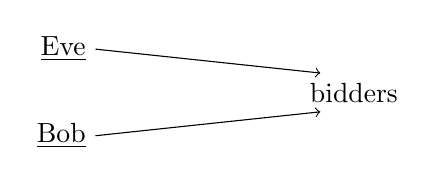
\begin{tikzpicture}[every node/.style={font=\normalsize}]
    \node[anchor=east] (eve) at (0,0.55) {\underline{Eve}};
    \node[anchor=east] (bob) at (0,-0.55) {\underline{Bob}};
    \node[anchor=west] (bid) at (2.6,0) {bidders};
    \draw[->] (eve.east) -- (bid.150);
    \draw[->] (bob.east) -- (bid.210);
\end{tikzpicture}
\caption{Eve and Bob are the two bidders.}
\end{figure}

Eve's plan: whatever Bob bids, she wants to bid double that amount.

Let Bob's secret bid be $m_{B}=5$. Alice receives
\[
    C_{B}\equiv m_{B}^{7}\pmod{77}.
\]
% filled in: $5^{7}=78125\equiv 47\pmod{77}$, so $C_{B}\equiv 47$.
\begingroup\samepage
Eve takes $k=2$ and builds a ciphertext for twice the bid, using the
public exponent on the multiplier:
\begin{align*}
    C_{E}
    &\equiv 2^{e}\,C_{B}\pmod{N}\\
    &\equiv 2^{7}\cdot 47
     \equiv 10\pmod{77}.
\end{align*}
\endgroup
% FIX p.39: the notes label this ciphertext $m_{E}$. It is $C_{E}$.
Alice decrypts Bob's ciphertext and recovers his bid:
\[
    m_{B}
    \equiv C_{B}^{d}
    \equiv m_{B}^{7d}
    \equiv 5\pmod{N}.
\]
Decrypting Eve's ciphertext gives
\[
    M_{E}
    \equiv C_{E}^{d}
    \equiv 2\,m_{B}
    \equiv 10\pmod{N}.
\]
% FIX p.39: the notes write $C_{E}^{d}=2^{e}\,C_{B}^{e}$. The right-hand
% side is not the decryption; $C_{E}\equiv 2^{e}C_{B}$ decrypts to $2m_{B}$.
% (In this tiny modulus one also has $10^{7}\equiv 10\pmod{77}$, so the
% ciphertext residue and the plaintext happen to coincide.)
Without padding, Eve's bid is exactly double Bob's, and Alice cannot tell
that the second ciphertext was manufactured from the first.

Alice therefore demands a check digit. A bid is sent as the block
$\begin{array}{|c|c|}\hline m & 1\\\hline\end{array}$.
Then
\begin{align*}
    C_{B}
    &\equiv
    \Biggl(
        \begin{array}{|c|c|}
            \hline
            m & 1\\
            \hline
        \end{array}
    \Biggr)^{e}
    \pmod{N},\\[0.4em]
    C_{E}
    &\equiv
    2^{e}
    \Biggl(
        \begin{array}{|c|c|}
            \hline
            m & 1\\
            \hline
        \end{array}
    \Biggr)^{e}
    \equiv
    \Biggl(
        2\cdot
        \begin{array}{|c|c|}
            \hline
            m & 1\\
            \hline
        \end{array}
    \Biggr)^{e}
    \pmod{N}.
\end{align*}
The integer inside Eve's power is Bob's block multiplied by $2$. In the
schematic of the notes that product is a block ending in $0$,
\[
    \begin{array}{|c|c|}
        \hline
        m_{E} & 0\\
        \hline
    \end{array},
\]
rather than a block ending in the check digit $1$.
% FIX p.39: the notes equate $C_{E}$ itself with the block $|m_{E}|0|$.
% That block is the plaintext Eve's ciphertext decrypts to.
\end{example}

% --- page 40 ---

Alice decrypts Bob's ciphertext and sees the check digit she asked for:
\begin{align*}
    M_{B}
    &\equiv C_{B}^{d}\pmod{N}\\
    &\equiv
    \Biggl(
        \begin{array}{|c|c|}
            \hline
            m & 1\\
            \hline
        \end{array}
    \Biggr)^{ed}
    \equiv
    \begin{array}{|c|c|}
        \hline
        m & 1\\
        \hline
    \end{array}
    \pmod{N}.
\end{align*}
% FIX p.40: the first line was written $M_{B}\equiv C_{B}\pmod{N}$,
% without the decryption exponent. The next line has the exponent $ed$.
Bob's bid is accepted. Eve's ciphertext decrypts to
\begin{align*}
    C_{E}^{d}
    &\equiv
    \Biggl(
        \begin{array}{|c|c|c|}
            \hline
            2 & m & 1\\
            \hline
        \end{array}
    \Biggr)^{ed}
    \equiv
    \begin{array}{|c|c|}
        \hline
        2m & 0\\
        \hline
    \end{array}
    \pmod{N}.
\end{align*}
The check digit is no longer $1$, so Alice rejects Eve's bid.

Suppose the padding has $216$ digits. The chance that multiplication
leaves that same padding is
\[
    \frac{1}{2^{216}},
\]
which is insignificant.
% UNCLEAR p.40: the length is written ``216 digits'', but the probability
% is $1/2^{216}$ (the count one would write for $216$ bits). Left as written.

% ============================================================
\section{Digital Signatures}
% ============================================================

Encryption is about secrecy: the message should not leak. A digital
signature is about authenticity of the message and of the sender.

A physical signature does not give that guarantee. On a degree
certificate the same handwritten signature can be copied from one line
to another.

\begin{figure}[H]
\centering
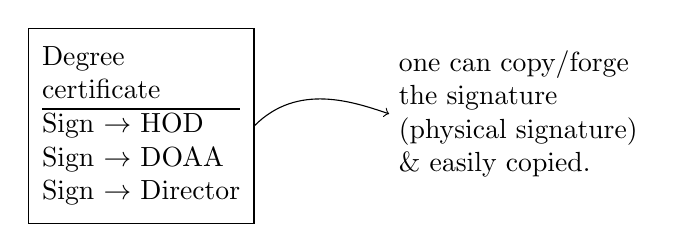
\begin{tikzpicture}[font=\normalsize]
    \node[draw, align=left, inner sep=5pt] (cert) at (0,0) {%
        \begin{tabular}{@{}l@{}}
            Degree\\
            certificate\\
            \hline
            Sign $\rightarrow$ HOD\\
            Sign $\rightarrow$ DOAA\\
            Sign $\rightarrow$ Director
        \end{tabular}};
    \node[align=left, anchor=west] (note) at (3.15,0.15)
        {one can copy/forge\\
         the signature\\
         (physical signature)\\
         \& easily copied.};
    \draw[->] (cert.east) .. controls +(0.55,0.55) and +(-0.45,0.15) .. (note.west);
\end{tikzpicture}
\caption{A physical signature on a degree certificate can be copied.}
\end{figure}

% --- page 41 ---

Three properties are required of a signature scheme.

\begin{enumerate}[leftmargin=1.6em]
    \item One wants an algorithm by which the signature cannot be copied
    or forged the way a physical signature can.

    \begin{figure}[H]
    \centering
    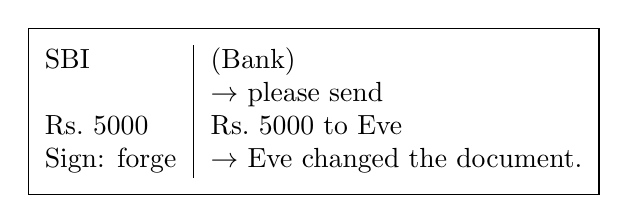
\begin{tikzpicture}[font=\normalsize]
        \node[draw, inner sep=6pt] {%
            \begin{tabular}{@{}l|l@{}}
                SBI & (Bank)\\
                & $\rightarrow$ please send\\
                Rs.\ 5000 & Rs.\ 5000 to Eve\\
                Sign: forge & $\rightarrow$ Eve changed the document.
            \end{tabular}};
    \end{tikzpicture}
    \caption{A forged signature on an altered bank instruction.}
    \end{figure}
    % UNCLEAR p.41: the amount cell reads roughly ``SSS 5000'' with a
    % rupee-like mark. Taken as Rs.\ 5000, and the annotation as
    % ``Rs.\ 5000 to Eve''.

    The picture is an instruction to SBI. Eve alters the document so that
    it says ``please send Rs.\ 5000 to Eve'' and forges the signature. A
    digital signature has to make that alteration detectable.

    \item In the signed copy, one cannot change the message. If Eve's
    change succeeds and the bank has transferred the money to Eve's
    account, Alice can deny that she signed the document. The signature
    must bind her to the text that was actually signed.

    \item \emph{Non-repudiation}: once Alice has signed, she cannot later
    deny the signature.
\end{enumerate}

% ------------------------------------------------------------
\subsection{RSA signatures}
% ------------------------------------------------------------

\begin{keybox}[title=RSA signatures]
\paragraph{Key generation (Alice).}
Alice chooses primes $p$ and $q$, sets $N=pq$, and chooses a verification
exponent $e$ with $\gcdop(e,\varphi(N))=1$. The signing exponent $d$ is
the inverse of $e$ modulo $\varphi(N)$, so $ed\equiv 1\pmod{\varphi(N)}$.
The public verification key is $(N,e)$; the private signing key is $d$.
Signing the document requires the private key.

% --- page 42 ---

Let $D$ be the document Alice wants to sign, read as an integer modulo $N$.

\paragraph{Signing.}
Alice computes
\[
    D^{\mathrm{sign}}\equiv D^{d}\pmod{N}
\]
and sends the pair $(D,D^{\mathrm{sign}})$ to Bob.

\paragraph{Verification.}
Bob computes $(D^{\mathrm{sign}})^{e}\pmod{N}$. Since
$ed\equiv 1\pmod{\varphi(N)}$,
\[
    (D^{\mathrm{sign}})^{e}
    \equiv D^{de}
    \equiv D\pmod{N}
\]
whenever $\gcdop(D,N)=1$. He accepts the signature when the power equals
$D$, and rejects it otherwise:
\[
    (D^{\mathrm{sign}})^{e}
    \equiv
    \begin{cases}
        D\pmod{N} & \text{true (accept)},\\
        \neq D\pmod{N} & \text{false (reject)}.
    \end{cases}
\]
\end{keybox}

\begin{example}[A small RSA signature]
Take $p=5$, $q=11$, so $N=55$ and $\varphi(N)=40$. Let $e=3$ and let the
document be $D=7$. The notes ask to verify the scheme on these values.

The signing exponent satisfies $3d\equiv 1\pmod{40}$. Since
$3\cdot 27=81\equiv 1\pmod{40}$, one may take $d=27$. Then
\begin{align*}
    7^{2}&\equiv 49,\\
    7^{3}&\equiv 13,\\
    7^{6}&\equiv 13^{2}=169\equiv 4,\\
    7^{12}&\equiv 16,\\
    7^{24}&\equiv 256\equiv 36\pmod{55},
\end{align*}
and
\[
    D^{\mathrm{sign}}
    \equiv 7^{27}
    \equiv 7^{24}\cdot 7^{2}\cdot 7
    \equiv 36\cdot 49\cdot 7
    \equiv 28\pmod{55}.
\]
Verification:
\[
    28^{3}=21952\equiv 7\pmod{55},
\]
which equals $D$, so Bob accepts.
% filled in: the notes set $p,q,N,\varphi(N),e,D$ and say ``verify'',
% without computing $d$ or $D^{\mathrm{sign}}$.
\end{example}

% ------------------------------------------------------------
\subsection{ElGamal signatures}
% ------------------------------------------------------------

In practice one uses a modified ElGamal signature, the Digital Signature
Algorithm (DSA), to sign documents.
% FIX p.42: the notes expand DSA as ``Digital Signing Algorithm''.

The construction is based on the discrete logarithm, as opposed to the
RSA power. The contrast drawn on the page is
\begin{align*}
    x^{e}&\equiv C\pmod{N}
        &&\text{is the RSA relation},\\
    g^{x}&\equiv C\pmod{N}
        &&\text{is the discrete-logarithm relation}.
\end{align*}

% --- page 43 ---

The signature reuses ElGamal encryption from Lecture~12: Bob sends and Alice receives.

\paragraph{Key generation.}
Alice chooses a large prime $p$, a base $g\in\units{p}$ of large order, and a private exponent $a\in\Z$. She computes
\[
    A\equiv g^{a}\pmod{p},
\]
publishes the public key $(A,g,p)$, and keeps the private key $a$.

\paragraph{Encryption.}
For a message $m$, Bob chooses an exponent $b$ satisfying
\[
    1<b\le p-1,
    \qquad
    \gcdop(b,p-1)=1,
\]
computes
\begin{align*}
    c_{1}&\equiv g^{b}\pmod{p},\\
    c_{2}&\equiv m\,A^{b}\pmod{p},
\end{align*}
and sends $(c_{1},c_{2})$ to Alice.

\paragraph{Decryption.}
Alice computes $x\equiv c_{1}^{a}\pmod{p}$ and $x^{-1}\pmod{p}$. Then
\begin{align*}
    x^{-1}c_{2}
    &\equiv c_{1}^{-a}\,m\,A^{b}
     \equiv g^{-ab}\,m\,g^{ab}
     \equiv m\pmod{p}.
\end{align*}
% p.43: board says ``large order'', public key $(A,g,p)$, and $a\in\Z$
% with no written range. Bob's exponent is $1<b\le p-1$ and $\gcd(b,p-1)=1$.

% --- page 44 ---

\paragraph{Signing a document.}
\begin{enumerate}[leftmargin=1.6em]
    \item Alice chooses $(p,g,a)$ as above, publishes $(A,p,g)$, and
    keeps $a$.

    \item To sign a document $D$ with $1<D<p$, she chooses an integer $k$
    satisfying
    \[
        \gcdop(k,p-1)=1,
        \qquad
        1<k<p,
    \]
    and sets
    \begin{align*}
        s_{1}&\equiv g^{k}\pmod{p},\\
        s_{2}&\equiv (D-as_{1})\,k^{-1}\pmod{p-1}.
    \end{align*}
    The inverse exists because $k$ is coprime to $p-1$. She sends
    $(D,s_{1},s_{2})$ to Bob.

    \item Bob computes $A^{s_{1}}s_{1}^{s_{2}}\pmod{p}$ and compares it
    with $g^{D}$:
    \[
        A^{s_{1}}s_{1}^{s_{2}}
        \equiv
        \begin{cases}
            g^{D}\pmod{p} & \text{true (accept)},\\
            \neq g^{D}\pmod{p} & \text{false (reject)}.
        \end{cases}
    \]
\end{enumerate}

The test accepts an honestly produced signature. Indeed, writing the
exponents modulo $p-1$ and using $g^{p-1}\equiv 1\pmod{p}$,
\begin{align*}
    A^{s_{1}}s_{1}^{s_{2}}
    &\equiv (g^{a})^{s_{1}}(g^{k})^{s_{2}}
     \equiv g^{as_{1}+ks_{2}}\pmod{p}\\
    &\equiv g^{as_{1}+(D-as_{1})}
     \equiv g^{D}\pmod{p},
\end{align*}
because $ks_{2}\equiv D-as_{1}\pmod{p-1}$.
% filled in: the notes state the accept/reject test without this expansion.

\lectureheading{Lecture 19 (23/10/26)}

% ============================================================
\section{Factorization via a Difference of Squares}
% ============================================================

The aim is to write the composite modulus as a difference of squares.
From $x^{2}-y^{2}=(x+y)(x-y)$ one wants integers $a>b>0$ with
\[
    N=(a-b)(a+b)=a^{2}-b^{2}.
\]
The two factors are then $a-b$ and $a+b$.

% --- page 45 ---

One keeps a reasonable distance between $a$ and $b$: if they are very
close, then $a-b$ is small and the factorization is easy to find by
trying.

If $N$ itself is hard to write as a difference of two squares, try the
same idea on a multiple. For some positive integer $k$, write
\[
    kN=(a-b)(a+b)=a^{2}-b^{2}.
\]
Any prime factor of $N$ then divides $a-b$ or $a+b$, and
$\gcdop(N,a-b)$ or $\gcdop(N,a+b)$ can be a proper factor.

Equivalently, one looks for $a$ and $b$ with
\[
    a^{2}-b^{2}\equiv 0\pmod{N},
    \qquad\text{i.e.}\qquad
    a^{2}\equiv b^{2}\pmod{N},
\]
and $a\not\equiv \pm b\pmod{N}$. Searching for such a pair at random is
hard. The following strategy builds the congruence out of several easier
ones.

\paragraph{Step 1.}
Find integers $a_{1},\ldots,a_{n}$ such that
\[
    a_{i}^{2}\equiv c_{i}\pmod{N},
\]
and each $c_{i}$ has only small prime factors.

\paragraph{Step 2.}
Choose a subset of these relations, say
$a_{n_{1}},\ldots,a_{n_{k}}$, whose corresponding residues multiply to a
square:
\[
    c_{n_{1}}\cdots c_{n_{k}}=b^{2}
\]
for some integer $b$. The product of the $a_{n_{j}}$ then satisfies
\[
    a^{2}
    =(a_{n_{1}}\cdots a_{n_{k}})^{2}
    \equiv b^{2}\pmod{N},
    \qquad
    a\equiv a_{n_{1}}\cdots a_{n_{k}}\pmod{N}.
\]

\paragraph{Step 3.}
Compute $\gcdop(N,a-b)$ or $\gcdop(N,a+b)$. Either gcd is a factor of $N$.
It is a proper factor precisely when $a\not\equiv \pm b\pmod{N}$.

% --- page 46 ---

\begin{example}[$N=3589$]
Take $N=3589=37\cdot 97$, so $\sqrt{N}\approx 59.9$ and one starts the
search just above $60$.
\begin{align*}
    60^{2}&=3600\equiv 11\pmod{N},\\
    61^{2}&=3721\equiv 132=2^{2}\cdot 3\cdot 11\pmod{N},\\
    64^{2}&=4096\equiv 507=3\cdot 13^{2}\pmod{N}.
\end{align*}
The product of the three residues is a square:
\[
    (60\cdot 61\cdot 64)^{2}
    \equiv 2^{2}\cdot 3^{2}\cdot 11^{2}\cdot 13^{2}\pmod{N}.
\]
Hence
\begin{align*}
    a&\equiv 60\cdot 61\cdot 64\equiv 955\pmod{N},\\
    b&=2\cdot 3\cdot 11\cdot 13=858.
\end{align*}
% filled in: $60\cdot 61=3660\equiv 71$ and $71\cdot 64=4544\equiv 955\pmod{3589}$.
Now $a-b=955-858=97$, and
\[
    \gcdop(N,a-b)=\gcdop(3589,97)=97,
\]
which is a prime factor of $N$. The complementary factor is
$N/97=37$. Equivalently,
\[
    a+b=1813
    \qquad\text{and}\qquad
    \gcdop(N,a+b)=37.
\]
% filled in: the notes record only $\gcdop(N,a-b)=97$.
\end{example}

\begin{remark}
The gcd may be trivial: $\gcdop(a\pm b,N)\in\{1,N\}$. In that case the
pair $(a,b)$ came from a combination with $a\equiv \pm b\pmod{N}$, and
one tries a different combination of the $a_{i}$. The residues $c_{i}$
have to be chosen so that they have small prime factors; otherwise the
search for a product that is a square does not get off the ground.
\end{remark}

\begin{definition}[Smooth numbers]
Let $B\ge 2$ be an integer. An integer $n\ge 2$ is \emph{$B$-smooth} if
every prime factor of $n$ is at most $B$.
\end{definition}

% --- page 47 ---

\begin{example}[$7$-smooth numbers up to $40$]
The $7$-smooth integers from $2$ to $40$ are
\begin{align*}
    &2,3,4,5,6,7,8,9,10,12,14,15,16,18,20,\\
    &21,24,25,27,28,30,32,35,36,40.
\end{align*}
The integers from $2$ to $40$ that are not $7$-smooth are
\begin{align*}
    &11,13,17,19,22,23,26,29,31,33,34,\\
    &37,38,39.
\end{align*}
There are $25$ numbers in the first list and $14$ in the second.
\end{example}

These numbers have to be counted, for the following reason. Suppose
relations
\[
    a_{1}^{2}\equiv c_{1},\quad
    a_{2}^{2}\equiv c_{2},\quad
    \ldots,\quad
    a_{n}^{2}\equiv c_{n}\pmod{N}
\]
have been found, and each $c_{i}$ factors over a fixed set of small
primes. Let
\[
    \{p_{1},\ldots,p_{t}\}
\]
be the first $t$ primes (the factor base), and write
\[
    c_{i}=p_{1}^{e_{1i}}\cdots p_{t}^{e_{ti}},
    \qquad 1\le i\le n.
\]
A subset of the relations multiplies to a square precisely when there
are exponents $u_{i}\in\{0,1\}$ such that
\[
    c_{1}^{u_{1}}\cdots c_{n}^{u_{n}}
\]
is a square. The choice $u_{i}=0$ leaves $c_{i}$ out of the product, and
$u_{i}=1$ puts it in. Expanding the product,
\begin{align*}
    c_{1}^{u_{1}}\cdots c_{n}^{u_{n}}
    &=
    p_{1}^{u_{1}e_{11}+u_{2}e_{12}+\cdots+u_{n}e_{1n}}\\
    &\qquad\cdots\;
    p_{t}^{u_{1}e_{t1}+u_{2}e_{t2}+\cdots+u_{n}e_{tn}}.
\end{align*}

% --- page 48 ---

The product is a square if and only if every exponent is even:
\begin{align*}
    u_{1}e_{11}+u_{2}e_{12}+\cdots+u_{n}e_{1n}
        &\equiv 0\pmod{2},\\
    &\vdots\\
    u_{1}e_{t1}+u_{2}e_{t2}+\cdots+u_{n}e_{tn}
        &\equiv 0\pmod{2}.
\end{align*}
This is a homogeneous linear system of $t$ equations in the $n$ unknowns
$u_{1},\ldots,u_{n}$, over the field $\Z/2\Z$. A homogeneous system with
more unknowns than equations has a non-trivial solution, so a non-trivial
solution exists whenever $n>t$.

The factor base is the set of the first $t$ primes, and $p_{t}$ is the
$t$-th prime, so $\pi(p_{t})=t$. The same demand can therefore be written
\[
    n>\pi(p_{t}):
\]
one needs more smooth relations than there are primes up to the
smoothness bound. To know whether a chosen bound produces that many
relations, one needs a count of smooth numbers.

\begin{definition}[Smooth-number counting function]
For $x\ge 1$ and an integer $B\ge 2$,
\[
    \psi(x,B)
    =
    \#\{\,n : 1<n\le x,\ n\text{ is $B$-smooth}\,\}.
\]
\end{definition}

\begin{example}
From the lists above, $\psi(20,7)=15$ and $\psi(40,7)=25$.
\end{example}

The two arguments have to be related before the count is useful as an
estimate. If $B>x$, every integer $n$ with $2\le n\le x$ is $B$-smooth,
because every prime factor of $n$ is at most $n\le x<B$. The definition
excludes $n=1$, so
\[
    \psi(x,B)=x-1
    \qquad\text{whenever }B>x
\]
(and $x$ is an integer). In the factorization one varies $x$ and $B$
together. Set
\[
    u=\frac{\log x}{\log B},
    \qquad\text{equivalently}\qquad
    B=x^{1/u}.
\]

% --- page 49 ---

\begin{keybox}
\begin{theorem}[Canfield--Erd\H{o}s--Pomerance]
Fix $0<\varepsilon<1/2$, and let $x$ and $B$ satisfy
\[
    (\log x)^{\varepsilon}
    <
    \log B
    <
    (\log x)^{1-\varepsilon}.
\]
Let $u=\log x/\log B$. Then
\[
    \psi(x,B)
    =
    x\,u^{-u\bigl(1+o(1)\bigr)}
    \qquad\text{as }x\to\infty.
\]
\end{theorem}
\end{keybox}
% FIX p.49: the notes spell the first name ``Caufield''.

\begin{remark}
The symbol $o(1)$ stands for a function of $x$ which tends to $0$ as
$x\to\infty$.
\end{remark}

To use $\psi(x,B)$ one still has to choose $B$. Define
\[
    L(x)
    =
    \exp\Bigl(\sqrt{\log x\cdot\log\log x}\Bigr).
\]
For every $m>0$ and every $\delta>0$, and for all sufficiently large $x$,
\[
    (\log x)^{m}<L(x)<x^{\delta}.
\]
% FIX p.49: the notes write both bounds with the side condition ``for $m>0$''
% and do not quantify $\delta$. The upper bound holds for every $\delta>0$.
In the order of growth this is the sandwich
\[
    (\log x)^{m}
    \;<\;
    \square
    \;<\;
    x^{\delta},
\]
with $L(x)$ an example of the middle term. A quantity of that shape is
called \emph{sub-exponential}.

\begin{figure}[H]
\centering
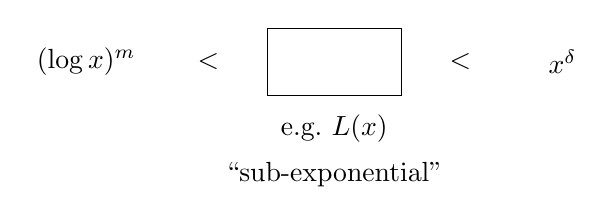
\begin{tikzpicture}[font=\normalsize]
    \node (left) at (0,0) {$(\log x)^{m}$};
    \node at (1.55,0) {$<$};
    \node[draw, minimum width=1.7cm, minimum height=0.85cm] (box) at (3.15,0) {};
    \node at (4.75,0) {$<$};
    \node (right) at (6.05,0) {$x^{\delta}$};
    \node[anchor=north] at (3.15,-0.55) {e.g.\ $L(x)$};
    \node[anchor=north] at (3.15,-1.15) {``sub-exponential''};
\end{tikzpicture}
\caption{Order of growth: $(\log x)^{m}<\square<x^{\delta}$, with $L(x)$ sub-exponential.}
\end{figure}

\begin{corollary}
For any $0<c<1$,
\[
    \psi\bigl(x,\,L(x)^{c}\bigr)
    =
    x\cdot L(x)^{-\frac{1}{2c}\bigl(1+o(1)\bigr)}.
\]
\end{corollary}

\begin{proof}
Set $B=L(x)^{c}$. Then
\begin{align*}
    \log B
    &= c\log L(x)\\
    &= c\sqrt{\log x\cdot\log\log x}.
\end{align*}
The notes record that this choice sits in a range to which the theorem
applies: for any $\varepsilon<1/2$,
\[
    \sqrt{\log x}
    <
    \log B
    <
    (\log x)^{1-\varepsilon}.
\]
For $\varepsilon<1/2$ and $x$ large, $(\log x)^{\varepsilon}<\sqrt{\log x}$, so the
same comparison puts $\log B$ between $(\log x)^{\varepsilon}$ and
$(\log x)^{1-\varepsilon}$.
% PROOF CONTINUES in part5; \end{proof} is there so the tombstone
% follows the finished argument rather than this page break.

